\subsection*{آ)}

دستور زبان مستقل از متن برابر است با:
\begin{eqnarray*}
    S &\rightarrow& S_1 | S_2 \\
    S_1 &\rightarrow& S_1c | A | \epsilon \\
    A &\rightarrow& aAb| \epsilon \\
    S_2 &\rightarrow& aS_2 | B | \epsilon \\
    B &\rightarrow& bBc|\epsilon 
\end{eqnarray*}

دقت کنید که A رشته‌ای با تعداد برابر a و b می‌سازد. همچنین B نیز رشته‌ای با تعداد برابر b و c می‌سازد. حالت دیگر این گرامر را می‌توان به شکل زیر نوشت که با هم معادل هستند.

\begin{eqnarray*}
    S &\rightarrow& S_1C|AS_2 \\
    S_1 &\rightarrow& aS_1b|\epsilon\\
    A &\rightarrow& aA|\epsilon\\
    S_2 &\rightarrow& bS_2c|\epsilon\\
    C &\rightarrow& cC|\epsilon
\end{eqnarray*}

خودکاره پشته‌ای متناظر به این زبان برابر است با:

\begin{center}
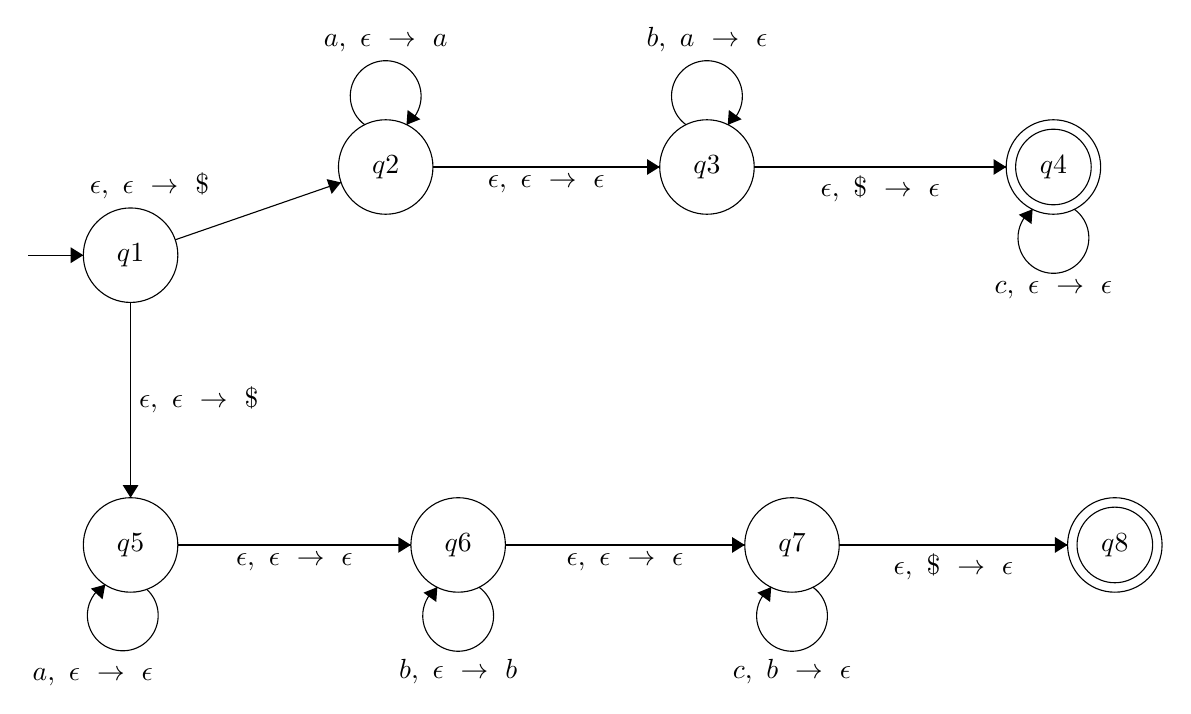
\begin{tikzpicture}[scale=0.2]
\tikzstyle{every node}+=[inner sep=0pt]
\draw [black] (12.8,-17.3) circle (3);
\draw (12.8,-17.3) node {$q1$};
\draw [black] (29,-11.7) circle (3);
\draw (29,-11.7) node {$q2$};
\draw [black] (12.8,-35.7) circle (3);
\draw (12.8,-35.7) node {$q5$};
\draw [black] (49.4,-11.7) circle (3);
\draw (49.4,-11.7) node {$q3$};
\draw [black] (71.4,-11.7) circle (3);
\draw (71.4,-11.7) node {$q4$};
\draw [black] (71.4,-11.7) circle (2.4);
\draw [black] (33.6,-35.7) circle (3);
\draw (33.6,-35.7) node {$q6$};
\draw [black] (54.8,-35.7) circle (3);
\draw (54.8,-35.7) node {$q7$};
\draw [black] (75.3,-35.7) circle (3);
\draw (75.3,-35.7) node {$q8$};
\draw [black] (75.3,-35.7) circle (2.4);
\draw [black] (6.3,-17.3) -- (9.8,-17.3);
\fill [black] (9.8,-17.3) -- (9,-16.8) -- (9,-17.8);
\draw [black] (15.64,-16.32) -- (26.16,-12.68);
\fill [black] (26.16,-12.68) -- (25.25,-12.47) -- (25.57,-13.41);
\draw (14,-13.75) node [above] {$\epsilon,\mbox{ }\epsilon\mbox{ }\rightarrow\mbox{ }\$$};
\draw [black] (32,-11.7) -- (46.4,-11.7);
\fill [black] (46.4,-11.7) -- (45.6,-11.2) -- (45.6,-12.2);
\draw (39.2,-12.2) node [below] {$\epsilon,\mbox{ }\epsilon\mbox{ }\rightarrow\mbox{ }\epsilon$};
\draw [black] (48.077,-9.02) arc (234:-54:2.25);
\draw (49.4,-4.45) node [above] {$b,\mbox{ }a\mbox{ }\rightarrow\mbox{ }\epsilon$};
\fill [black] (50.72,-9.02) -- (51.6,-8.67) -- (50.79,-8.08);
\draw [black] (13.819,-38.509) arc (47.65981:-240.34019:2.25);
\draw (10.4,-43.53) node [below] {$a,\mbox{ }\epsilon\mbox{ }\rightarrow\mbox{ }\epsilon$};
\fill [black] (11.19,-38.22) -- (10.28,-38.47) -- (11.02,-39.15);
\draw [black] (27.677,-9.02) arc (234:-54:2.25);
\draw (29,-4.45) node [above] {$a,\mbox{ }\epsilon\mbox{ }\rightarrow\mbox{ }a$};
\fill [black] (30.32,-9.02) -- (31.2,-8.67) -- (30.39,-8.08);
\draw [black] (12.8,-20.3) -- (12.8,-32.7);
\fill [black] (12.8,-32.7) -- (13.3,-31.9) -- (12.3,-31.9);
\draw (13.3,-26.5) node [right] {$\epsilon,\mbox{ }\epsilon\mbox{ }\rightarrow\mbox{ }\$$};
\draw [black] (52.4,-11.7) -- (68.4,-11.7);
\fill [black] (68.4,-11.7) -- (67.6,-11.2) -- (67.6,-12.2);
\draw (60.4,-12.2) node [below] {$\epsilon,\mbox{ }\$\mbox{ }\rightarrow\mbox{ }\epsilon$};
\draw [black] (72.723,-14.38) arc (54:-234:2.25);
\draw (71.4,-18.95) node [below] {$c,\mbox{ }\epsilon\mbox{ }\rightarrow\mbox{ }\epsilon$};
\fill [black] (70.08,-14.38) -- (69.2,-14.73) -- (70.01,-15.32);
\draw [black] (15.8,-35.7) -- (30.6,-35.7);
\fill [black] (30.6,-35.7) -- (29.8,-35.2) -- (29.8,-36.2);
\draw (23.2,-36.2) node [below] {$\epsilon,\mbox{ }\epsilon\mbox{ }\rightarrow\mbox{ }\epsilon$};
\draw [black] (34.923,-38.38) arc (54:-234:2.25);
\draw (33.6,-42.95) node [below] {$b,\mbox{ }\epsilon\mbox{ }\rightarrow\mbox{ }b$};
\fill [black] (32.28,-38.38) -- (31.4,-38.73) -- (32.21,-39.32);
\draw [black] (36.6,-35.7) -- (51.8,-35.7);
\fill [black] (51.8,-35.7) -- (51,-35.2) -- (51,-36.2);
\draw (44.2,-36.2) node [below] {$\epsilon,\mbox{ }\epsilon\mbox{ }\rightarrow\mbox{ }\epsilon$};
\draw [black] (56.123,-38.38) arc (54:-234:2.25);
\draw (54.8,-42.95) node [below] {$c,\mbox{ }b\mbox{ }\rightarrow\mbox{ }\epsilon$};
\fill [black] (53.48,-38.38) -- (52.6,-38.73) -- (53.41,-39.32);
\draw [black] (57.8,-35.7) -- (72.3,-35.7);
\fill [black] (72.3,-35.7) -- (71.5,-35.2) -- (71.5,-36.2);
\draw (65.05,-36.2) node [below] {$\epsilon,\mbox{ }\$\mbox{ }\rightarrow\mbox{ }\epsilon$};
\end{tikzpicture}
\end{center}

\subsection*{ب)}

دستور زبان مستقل از متن برابر است با:
\begin{eqnarray*}
    S &\rightarrow& SS \;|\; (S)\; |\; [S]\; | \epsilon \\
\end{eqnarray*}

خودکاره پشته‌ای متناظر به این زبان برابر است با:

\begin{center}
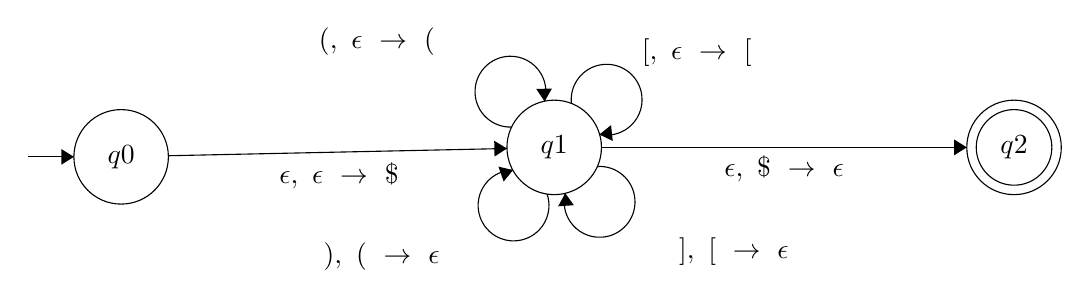
\begin{tikzpicture}[scale=0.2]
\tikzstyle{every node}+=[inner sep=0pt]
\draw [black] (11.4,-25.3) circle (3);
\draw (11.4,-25.3) node {$q0$};
\draw [black] (38.9,-24.7) circle (3);
\draw (38.9,-24.7) node {$q1$};
\draw [black] (68.1,-24.7) circle (3);
\draw (68.1,-24.7) node {$q2$};
\draw [black] (68.1,-24.7) circle (2.4);
\draw [black] (14.4,-25.23) -- (35.9,-24.77);
\fill [black] (35.9,-24.77) -- (35.09,-24.28) -- (35.11,-25.28);
\draw (25.23,-25.66) node [below] {$\epsilon,\mbox{ }\epsilon\mbox{ }\rightarrow\mbox{ }\$$};
\draw [black] (41.9,-24.7) -- (65.1,-24.7);
\fill [black] (65.1,-24.7) -- (64.3,-24.2) -- (64.3,-25.2);
\draw (53.5,-25.2) node [below] {$\epsilon,\mbox{ }\$\mbox{ }\rightarrow\mbox{ }\epsilon$};
\draw [black] (36.205,-23.409) arc (272.1282:-15.8718:2.25);
\draw (27.64,-18.89) node [above] {$(,\mbox{ }\epsilon\mbox{ }\rightarrow\mbox{ }($};
\fill [black] (38.29,-21.78) -- (38.76,-20.96) -- (37.76,-20.99);
\draw [black] (38.445,-27.654) arc (18.98162:-269.01838:2.25);
\draw (27.94,-30.73) node [below] {$),\mbox{ }(\mbox{ }\rightarrow\mbox{ }\epsilon$};
\fill [black] (36.28,-26.14) -- (35.36,-25.92) -- (35.69,-26.87);
\draw [black] (39.993,-21.919) arc (186.27369:-101.72631:2.25);
\draw (44.43,-18.7) node [right] {$[,\mbox{ }\epsilon\mbox{ }\rightarrow\mbox{ }[$};
\fill [black] (41.77,-23.88) -- (42.62,-24.29) -- (42.51,-23.29);
\draw [black] (41.631,-25.912) arc (93.80557:-194.19443:2.25);
\draw (50.31,-30.38) node [below] {$],\mbox{ }[\mbox{ }\rightarrow\mbox{ }\epsilon$};
\fill [black] (39.6,-27.61) -- (39.15,-28.44) -- (40.15,-28.37);
\draw [black] (5.5,-25.3) -- (8.4,-25.3);
\fill [black] (8.4,-25.3) -- (7.6,-24.8) -- (7.6,-25.8);
\end{tikzpicture}
\end{center}

\subsection*{ج)}

گرامر این زبان برابر است با:

\begin{eqnarray*}
    S &\rightarrow& aSb \;|\; aaSb\; |\; aaSbbb\; |\; \epsilon \\
\end{eqnarray*}
 دقت کنید می‌خوهیم که 
 $i \leq 2j \leq 3i$ باشد. 
 قاعده اول تعداد برابر a و b تولید می‌کند که در زبان بیان شده است.
 قاعده دوم به ما کمک می‌کند تا رشته‌هایی که 2 برابر تعداد b های آن با تعداد aهایش برابر است ایجاد بشود. 
 قاعده سوم نیز بررسی می‌کند تا  2 برابر تعداد b ها با 3 برابر تعداد a ها برابر شود. 
 حال با ترکیب این 3 قاعده، به گرامر زبان مورد نظر می‌رسیم. چون تعداد b ها هیچ‌گاه 2 برابر تعداد a ها و یا کمتر از نصف آنها نمی‌شود.\\
حال طبق مثال زیر از سورس، گرامر را به pda تبدیل می‌کنیم.
\begin{figure} [H]
    \centering
    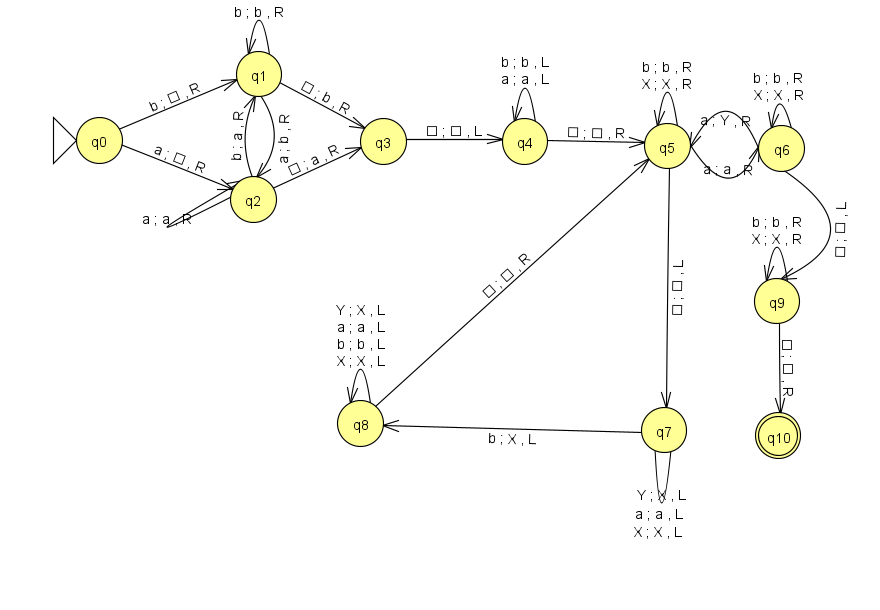
\includegraphics[scale=0.8]{solution/1-3.png}
\end{figure}

داریم
( دقت کنید مرحله پوش کردن $\$$ و s با هم انجام شده است.) :

\begin{center}
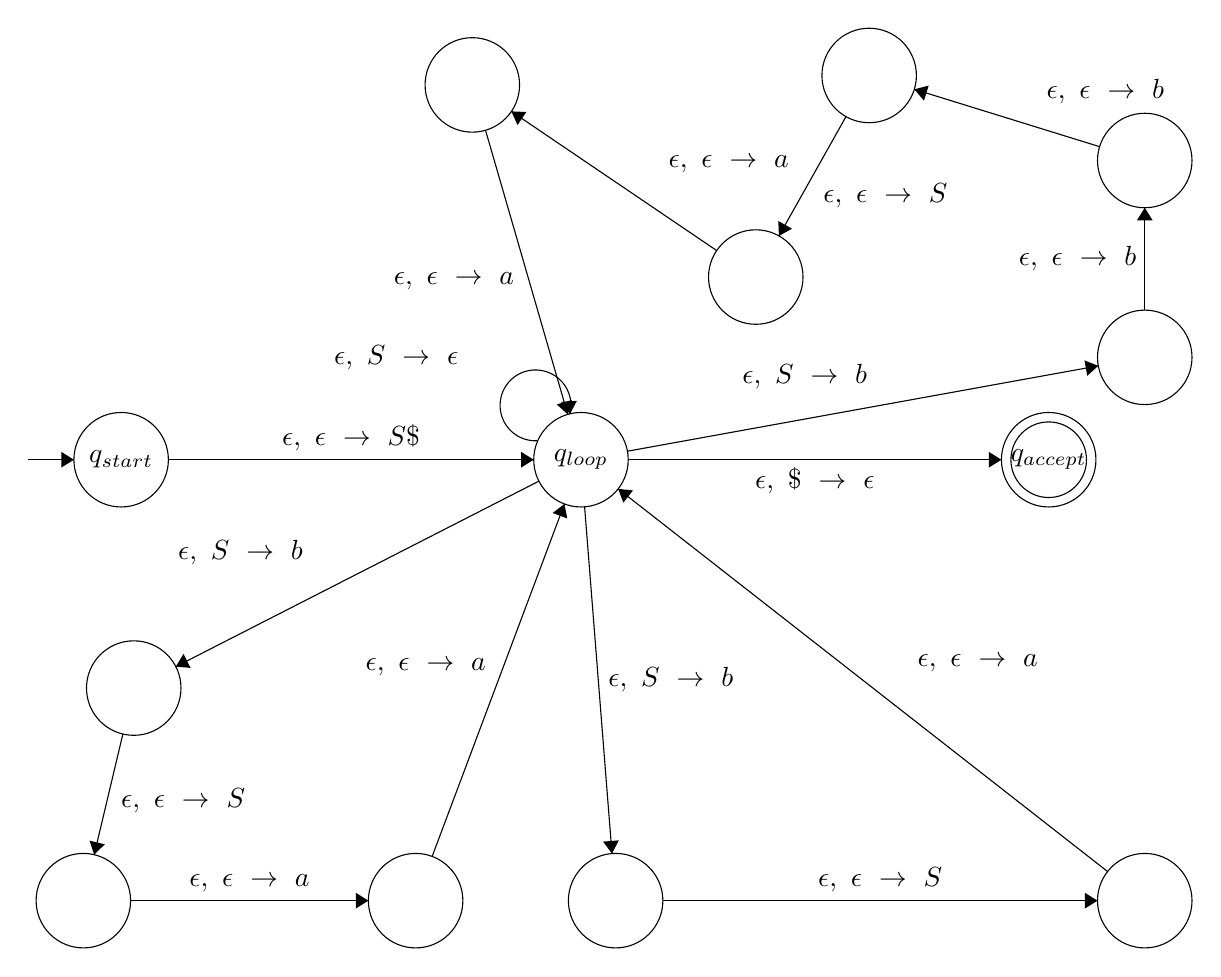
\begin{tikzpicture}[scale=0.2]
\tikzstyle{every node}+=[inner sep=0pt]
\draw [black] (9.4,-27.8) circle (3);
\draw (9.4,-27.8) node {$q_{start}$};
\draw [black] (38.6,-27.8) circle (3);
\draw (38.6,-27.8) node {$q_{loop}$};
\draw [black] (68.3,-27.8) circle (3);
\draw (68.3,-27.8) node {$q_{accept}$};
\draw [black] (68.3,-27.8) circle (2.4);
\draw [black] (10.2,-42.3) circle (3);
\draw [black] (7,-55.8) circle (3);
\draw [black] (28.1,-55.8) circle (3);
\draw [black] (40.8,-55.8) circle (3);
\draw [black] (74.4,-55.8) circle (3);
\draw [black] (74.4,-21.3) circle (3);
\draw [black] (74.4,-8.8) circle (3);
\draw [black] (56.9,-3.4) circle (3);
\draw [black] (49.7,-16.2) circle (3);
\draw [black] (31.7,-4) circle (3);
\draw [black] (12.4,-27.8) -- (35.6,-27.8);
\fill [black] (35.6,-27.8) -- (34.8,-27.3) -- (34.8,-28.3);
\draw (24,-27.3) node [above] {$\epsilon,\mbox{ }\epsilon\mbox{ }\rightarrow\mbox{ }S\$$};
\draw [black] (41.6,-27.8) -- (65.3,-27.8);
\fill [black] (65.3,-27.8) -- (64.5,-27.3) -- (64.5,-28.3);
\draw (53.45,-28.3) node [below] {$\epsilon,\mbox{ }\$\mbox{ }\rightarrow\mbox{ }\epsilon$};
\draw [black] (3.5,-27.8) -- (6.4,-27.8);
\fill [black] (6.4,-27.8) -- (5.6,-27.3) -- (5.6,-28.3);
\draw [black] (35.93,-29.16) -- (12.87,-40.94);
\fill [black] (12.87,-40.94) -- (13.81,-41.02) -- (13.36,-40.13);
\draw (16.98,-34.52) node [above] {$\epsilon,\mbox{ }S\mbox{ }\rightarrow\mbox{ }b$};
\draw [black] (9.51,-45.22) -- (7.69,-52.88);
\fill [black] (7.69,-52.88) -- (8.36,-52.22) -- (7.39,-51.99);
\draw (9.36,-49.47) node [right] {$\epsilon,\mbox{ }\epsilon\mbox{ }\rightarrow\mbox{ }S$};
\draw [black] (10,-55.8) -- (25.1,-55.8);
\fill [black] (25.1,-55.8) -- (24.3,-55.3) -- (24.3,-56.3);
\draw (17.55,-55.3) node [above] {$\epsilon,\mbox{ }\epsilon\mbox{ }\rightarrow\mbox{ }a$};
\draw [black] (29.15,-52.99) -- (37.55,-30.61);
\fill [black] (37.55,-30.61) -- (36.8,-31.18) -- (37.73,-31.53);
\draw (32.59,-40.98) node [left] {$\epsilon,\mbox{ }\epsilon\mbox{ }\rightarrow\mbox{ }a$};
\draw [black] (35.866,-26.593) arc (273.9076:-14.0924:2.25);
\draw (26.87,-22.13) node [above] {$\epsilon,\mbox{ }S\mbox{ }\rightarrow\mbox{ }\epsilon$};
\fill [black] (37.9,-24.9) -- (38.34,-24.06) -- (37.34,-24.13);
\draw [black] (38.83,-30.79) -- (40.57,-52.81);
\fill [black] (40.57,-52.81) -- (41,-51.97) -- (40,-52.05);
\draw (40.31,-41.75) node [right] {$\epsilon,\mbox{ }S\mbox{ }\rightarrow\mbox{ }b$};
\draw [black] (43.8,-55.8) -- (71.4,-55.8);
\fill [black] (71.4,-55.8) -- (70.6,-55.3) -- (70.6,-56.3);
\draw (57.6,-55.3) node [above] {$\epsilon,\mbox{ }\epsilon\mbox{ }\rightarrow\mbox{ }S$};
\draw [black] (72.04,-53.95) -- (40.96,-29.65);
\fill [black] (40.96,-29.65) -- (41.29,-30.53) -- (41.9,-29.75);
\draw (63.79,-41.3) node [above] {$\epsilon,\mbox{ }\epsilon\mbox{ }\rightarrow\mbox{ }a$};
\draw [black] (41.55,-27.26) -- (71.45,-21.84);
\fill [black] (71.45,-21.84) -- (70.57,-21.49) -- (70.75,-22.47);
\draw (52.81,-23.36) node [above] {$\epsilon,\mbox{ }S\mbox{ }\rightarrow\mbox{ }b$};
\draw [black] (74.4,-18.3) -- (74.4,-11.8);
\fill [black] (74.4,-11.8) -- (73.9,-12.6) -- (74.9,-12.6);
\draw (73.9,-15.05) node [left] {$\epsilon,\mbox{ }\epsilon\mbox{ }\rightarrow\mbox{ }b$};
\draw [black] (55.43,-6.01) -- (51.17,-13.59);
\fill [black] (51.17,-13.59) -- (52,-13.13) -- (51.13,-12.64);
\draw (53.96,-11.01) node [right] {$\epsilon,\mbox{ }\epsilon\mbox{ }\rightarrow\mbox{ }S$};
\draw [black] (47.22,-14.52) -- (34.18,-5.68);
\fill [black] (34.18,-5.68) -- (34.57,-6.55) -- (35.13,-5.72);
\draw (47.98,-9.6) node [above] {$\epsilon,\mbox{ }\epsilon\mbox{ }\rightarrow\mbox{ }a$};
\draw [black] (32.54,-6.88) -- (37.76,-24.92);
\fill [black] (37.76,-24.92) -- (38.02,-24.01) -- (37.06,-24.29);
\draw (34.38,-16.48) node [left] {$\epsilon,\mbox{ }\epsilon\mbox{ }\rightarrow\mbox{ }a$};
\draw [black] (71.53,-7.92) -- (59.77,-4.28);
\fill [black] (59.77,-4.28) -- (60.38,-5) -- (60.68,-4.04);
\draw (71.9,-5.26) node [above] {$\epsilon,\mbox{ }\epsilon\mbox{ }\rightarrow\mbox{ }b$};
\end{tikzpicture}
\end{center}

